\documentclass[10pt,a4paper]{article}
\usepackage[a4paper,margin=1.8cm,top=1.5cm,bottom=1.6cm]{geometry}
\usepackage[T1]{fontenc}
\usepackage{lmodern}
\usepackage{microtype}
\usepackage{booktabs,tabularx,array}
\usepackage{enumitem}
\usepackage{titlesec}
\usepackage{xcolor}
\usepackage{graphicx}
\usepackage{caption,subcaption}
\usepackage{float}
\usepackage[hidelinks]{hyperref}
\usepackage{mdframed}
\usepackage{amsmath}
\usepackage{tikz}
\usetikzlibrary{positioning,arrows.meta,calc}

\setlist[itemize]{leftmargin=1.2em,itemsep=1pt,topsep=2pt,parsep=0pt}
\titleformat{\section}{\large\bfseries}{\thesection.}{0.5em}{}
\titlespacing*{\section}{0pt}{9pt}{3pt}
\titleformat{\subsection}{\normalsize\bfseries}{\thesubsection}{0.5em}{}
\titlespacing*{\subsection}{0pt}{6pt}{2pt}
\setlength{\parindent}{0pt}
\setlength{\parskip}{3pt}
\renewcommand{\arraystretch}{1.12}
\newcolumntype{Y}{>{\raggedright\arraybackslash}X}
\captionsetup{font=small,labelfont=bf,skip=3pt}
\setlength{\textfloatsep}{8pt}
\setlength{\floatsep}{6pt}
\setlength{\intextsep}{6pt}
\definecolor{cardbg}{HTML}{F2F5F4}
\definecolor{cardline}{HTML}{1F6F5C}

\begin{document}

\begin{center}
{\LARGE\bfseries Roostoo ML Intern Assignment}\\[4pt]
{\small Atharva Moghe \quad$\cdot$\quad Predictive ML Trading Assistant assessment \quad$\cdot$\quad 28 October 2026}\\[2pt]
{\small \href{mailto:cs23b096@smail.iitm.ac.in}{\texttt{cs23b096@smail.iitm.ac.in}} \quad$\cdot$\quad \href{mailto:mogheatharva16@gmail.com}{\texttt{mogheatharva16@gmail.com}} \quad$\cdot$\quad \texttt{+91 94915 61608}}\\[2pt]
{\small Code and full experiment log: \href{https://github.com/Atharva-Mog/Roostoo-Project}{\texttt{github.com/Atharva-Mog/Roostoo-Project}}}
\end{center}

\textbf{Goal.} Help a new BTC/USDT trader take \textbf{fewer and better trades}. Every 4 hours the agent answers four questions:
\emph{what is the market like, is a trade worth taking after my own fees, how big should it be and where do I exit, and should I
trust the agent right now?}
% The design was shaped by 19 logged
% experiments on 2021--2026 Binance data. Code, the full experiment log and an
% \href{https://claude.ai/artifact/7RN6eZzquGSWNQ6qn4xQjE}{\underline{interactive mock-up}} built from the agent's real replay accompany this plan.

\begin{figure}[H]
\centering
{\normalsize\bfseries\color{cardline} Model Flowchart}\\[4pt]
\begin{tikzpicture}[
  node distance=5mm,
  box/.style={draw=cardline, fill=cardbg, rounded corners=2pt, align=center, font=\scriptsize, minimum height=10mm, text width=25mm, inner sep=2pt},
  st/.style={draw=cardline, fill=white, rounded corners=1.5pt, font=\scriptsize\bfseries, inner sep=2pt, minimum height=5mm},
  arr/.style={-{Stealth[length=1.6mm]}, draw=cardline, line width=0.6pt}]
  \node[box] (obs) {\textbf{1. Observe}\\prices, funding,\\open interest, ETH};
  \node[box, right=of obs] (read) {\textbf{2. Read the market}\\volatility level,\\4-week trend};
  \node[box, right=of read] (pred) {\textbf{3. Predict}\\P(target), P(stop),\\P(neither), size of move};
  \node[box, right=of pred] (ev) {\textbf{4. Decide}\\expected value\\after \emph{your} fees};
  \node[box, right=of ev] (plan) {\textbf{5. Plan \& explain}\\stop, target, size,\\three reasons};
  \node[box, below=12mm of obs] (learn) {\textbf{6. Learn}\\resolve past signals,\\check calibration};
  \node[draw=cardline, line width=0.8pt, rounded corners=2pt, fill=white, inner sep=3pt,
        anchor=west] (card) at ($(learn.east)+(14mm,0)$) {%
    \begin{tikzpicture}[node distance=2mm]
      \node[font=\scriptsize\bfseries] (lbl) {Card to trader:};
      \node[st, right=of lbl, text=green!40!black] (t) {TAKE};
      \node[st, right=of t, text=orange!70!black] (s) {SKIP};
      \node[st, right=of s] (a) {STAND ASIDE};
      \node[st, right=of a, text=red!60!black] (p) {PAUSED};
    \end{tikzpicture}};
  \draw[arr] (obs) -- (read); \draw[arr] (read) -- (pred); \draw[arr] (pred) -- (ev); \draw[arr] (ev) -- (plan);
  \draw[arr] (plan.south) |- (card.east);
  \draw[arr] (card.west) -- node[below, font=\scriptsize]{outcomes} (learn.east);
  \draw[arr, dashed] (learn.north) -- node[right, font=\scriptsize, align=left, xshift=1mm]{next cycle in 4h; retrain monthly} (obs.south);
\end{tikzpicture}
\caption{\textbf{Model flowchart}: the agent's 4-hour decision cycle. Steps 1--5 turn the latest data into one card for the trader. Step 6 compares past
predictions with what actually happened: if they have drifted, the next cards are PAUSED until accuracy recovers; the model is
also retrained every month on newly resolved data.}
\label{fig:loop}
\end{figure}

\section{About the model}

\subsection{Prediction target and horizon}
\begin{itemize}
  \item \textbf{Target.} For a long entry now, \textbf{calibrated probabilities of three outcomes in the next 24 hours}:
        \emph{take-profit first} ($+1.5\sigma$), \emph{stop first} ($-1\sigma$), or \emph{neither}. $\sigma$ is the current
        typical 24h move, so the barriers scale with volatility.
  \item \textbf{Why it helps.} A beginner needs a \textbf{decision, not a forecast}. With the trader's own fees the probabilities give
        the \textbf{expected value of this trade for this trader},
        $\mathrm{EV} = (1.5\,p_{\mathrm{TP}} - p_{\mathrm{SL}} + \bar r_{\mathrm{TO}}\,p_{\mathrm{TO}})\,\sigma - \text{fees}$.
        Its sign decides \emph{take or skip}; the same $\sigma$ sets the stop, target and position size.
  \item \textbf{Horizon: 24h on 1h bars}, picked from a grid \emph{fixed in advance} (15m/1h/4h bars $\times$ 4h/12h/24h).
        24h was best at every bar size and 4h worst (Figure~\ref{fig:grid}a), exactly what fees predict.
\end{itemize}

\subsection{Data and features}
\begin{itemize}
  \item \textbf{Data.} Free \textbf{Binance} data, Jan 2021 -- Oct 2026: BTC and ETH spot (15 min), plus \emph{futures funding rates,
        open interest and long/short ratios}.
  \item \textbf{Features.} \textbf{39 features in six groups}, each a hypothesis. \textbf{Volatility} was strongest; \emph{order flow},
        \emph{futures positioning} (crowded leveraged longs) and \emph{ETH vs BTC} added value; short-term \emph{momentum} never did.
  \item \textbf{No leakage.} Features use only data available at that moment; feature selection is fitted on training folds only.
\end{itemize}

\subsection{Model and baseline}
\begin{itemize}
  \item \textbf{Model.} A \textbf{shallow three-class LightGBM} (depth 3), with weights for overlapping labels and
        \textbf{isotonic calibration}, because the decision compares a probability with a fee.
  \item \textbf{Why this model.} The inputs are \emph{tabular, mixed-scale and partly missing}, and the useful signals are
        \emph{interactions} (high funding \emph{and} rising open interest means a crowded market). \textbf{Gradient-boosted trees}
        handle all of this natively and retrain in seconds. They are kept \textbf{shallow} because there are only about
        \textbf{2,000 independent 24h outcomes}, where deep trees or neural networks would fit noise. \emph{Three classes} let EV
        account for stop-outs and trades that go nowhere.
  \item \textbf{Starting model.} \emph{Logistic regression}. LightGBM beat it only at 24h and only slightly on the
        final test ($-15.8\%$ vs $-17.9\%$), so logistic regression stays as the \textbf{fallback}. \emph{Note:} this comparison
        comes from our earlier runs on \textbf{Bitstamp} BTC/USD data with price and volume features only (Binance was not reachable
        at the time); logistic regression cannot handle the missing values in the later futures features, so it was not rerun on Binance.
  \item \textbf{Baselines.} Buy-and-hold, every trade, majority-class probabilities, a \textbf{random filter with the same number of
        trades}, \textbf{shuffled-label retrains}, and two published strategies (4-week trend, funding carry).
\end{itemize}

\subsection{Validation and backtest design}
\begin{itemize}
  \item \textbf{Walk-forward}: train on everything up to a date, test on the next 6 months, \textbf{8 periods} from mid-2022;
        overlapping labels are \emph{purged}; the \textbf{last 6 months held out}.
  \item \textbf{Realistic costs}: \textbf{0.25\% round trip} on spot; futures limit orders fill only if price trades through; funding charged.
  \item \textbf{Checks}: prediction and trading metrics reported separately, with \emph{bootstrap ranges}, a \emph{shuffled-label null}
        and a \emph{fee sweep}.
\end{itemize}
\textbf{Results.} Direction is \textbf{weak} (AUC $\approx 0.55$), but the \textbf{ranking of trades is real}: it beat 97\% of shuffled
retrains and held out of sample (Figure~\ref{fig:grid}b). The average edge (\textbf{0.09\%}) is \textbf{below beginner fees (0.25\%)};
breakeven is about 0.10\%. The best configuration \textbf{lost 29\% on the final 6 months}: the edge was strong in 2023--2024 and faded.

\begin{figure}[H]
  \centering
  \begin{subfigure}[t]{0.29\textwidth}\centering
    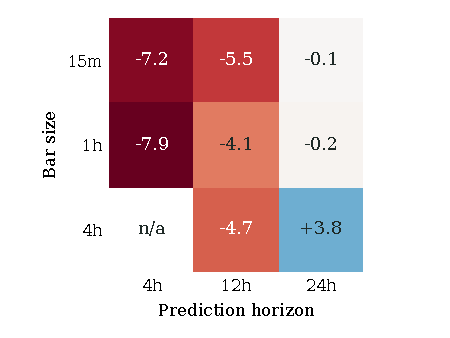
\includegraphics[width=\linewidth]{fig/fig_horizon.pdf}
    \caption{Net return per trade (bps).}
  \end{subfigure}\hspace{0.04\textwidth}
  \begin{subfigure}[t]{0.37\textwidth}\centering
    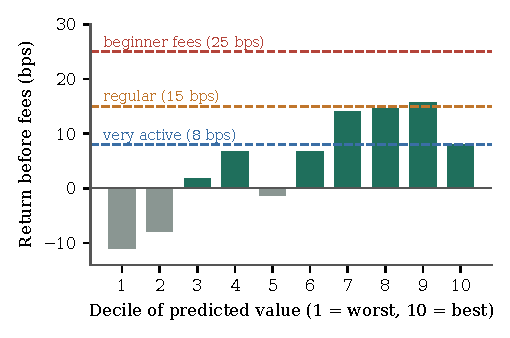
\includegraphics[width=\linewidth]{fig/fig_edge_fees.pdf}
    \caption{Pre-fee return by decile vs fee levels.}
  \end{subfigure}
  \caption{(a) Only the 24h horizon is near or above zero. (b) The model ranks trades (top deciles +14--16 bps before fees),
  but only a very-low-fee trader clears the bar.}
  \label{fig:grid}
\end{figure}

The model's \textbf{real strength is predicting the size of the next move}. A next-24h \textbf{volatility forecast beats every standard
baseline, including HAR-RV} (Table~\ref{tab:vol}, Figure~\ref{fig:vol}); trade-count surges, open-interest changes and ETH vs BTC are
top features that a price-only model cannot see. The coach uses it for \emph{stops, sizing and ``wild day'' warnings}.

\begin{table}[H]
\centering\small
\caption{Next-24h volatility forecasts (QLIKE loss, lower is better).}
\label{tab:vol}
\begin{tabular}{lcccc}
\toprule
Model & QLIKE, 8 periods & vs HAR & QLIKE, final 6m & $R^2$ (log), final 6m \\
\midrule
Yesterday's volatility & 0.493 & $-31\%$ & 0.374 & $-0.37$ \\
EWMA (3-day) & 0.437 & $-16\%$ & 0.304 & $-0.05$ \\
HAR-RV (benchmark) & 0.376 & -- & 0.274 & 0.01 \\
\textbf{LightGBM, our features} & \textbf{0.349} & \textbf{+7\%} ($t{=}1.6$) & \textbf{0.221} & \textbf{0.35} \\
\bottomrule
\end{tabular}
\end{table}

\begin{figure}[H]
  \centering
  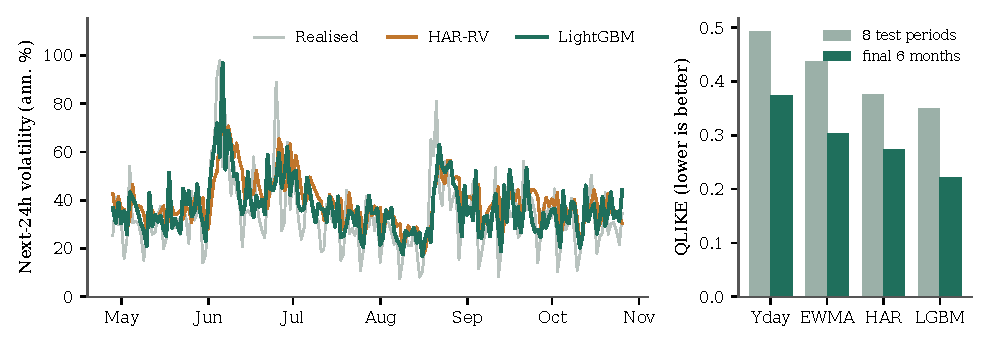
\includegraphics[width=0.8\textwidth]{fig/fig_vol.pdf}
  \caption{Realised vs forecast volatility (final 6 months) and forecast error by model. Gain over HAR: borderline over 8 periods,
  significant on the final 6 months ($+19\%$, $t{=}2.3$).}
  \label{fig:vol}
\end{figure}

\subsection{How the agent works and what the trader sees}
The output must be \textbf{simple}, since the user is new to crypto. Every 4 hours the agent runs the loop in Figure~\ref{fig:loop}.



Each card is in one of four states: \textbf{TAKE} (edge beats \emph{your} fees), \textbf{SKIP} (edge exists but fees remove it; the
card shows the fee level that would make it worthwhile), \textbf{STAND ASIDE} (no edge; hold in an uptrend, cash in a downtrend) or
\textbf{PAUSED} (recent predictions drifted from outcomes). A real card from the replay, for a regular trader:

\begin{mdframed}[backgroundcolor=cardbg,linecolor=cardline,linewidth=0pt,leftline=true,innerleftmargin=8pt,innertopmargin=4pt,innerbottommargin=4pt,skipabove=2pt,skipbelow=2pt]
\small
\textbf{TAKE --- leaning up for the next 24h.} Confidence: high (top 10\% of setups).\\
Odds: target first 12\%, stop first 11\%, neither 76\%. Expected +0.27\%, your fees 0.15\%, \textbf{net +0.12\%}.\\
Buy \$84,736 $\cdot$ take profit \$86,498 $\cdot$ stop \$83,581 $\cdot$ close after 24h $\cdot$ size 73\% of account (the stop costs 1\%).\\
Why: funding is low this month; ETH is lagging BTC; weekly volatility is low.
\end{mdframed}

The trader picks a \textbf{profile}, which changes which signals are shown and how they are sized:

\begin{table}[H]
\centering\small
\begin{tabularx}{\textwidth}{lYYY}
\toprule
 & Beginner & Regular & Very active \\
\midrule
Signals shown & Top 10\% confidence, clearly above fees & Medium and high confidence & Any edge after fees \\
Risk per trade & 0.5\%, at most half the account & 1\% & 1\% \\
Typical fees & 0.25\% spot & 0.15\% & 0.08\% futures \\
Falling markets & Cash; explains why not to short & Explains shorts only & Short view, no leverage \\
\textbf{Final 6 months, coach} & $\mathbf{-9.1\%}$ (20 trades) & $\mathbf{-3.5\%}$ (45 trades) & $\mathbf{-1.8\%}$ (68 trades) \\
Final 6 months, every signal & $-61\%$ & $-39\%$ & $-24\%$ \\
\bottomrule
\end{tabularx}
\end{table}

\textbf{Check my idea} grades the trader's own plan from A to D (\emph{chasing a pump, a stop inside normal noise, too much at risk}),
then shows what actually happened. A \textbf{weekly report} and a \textbf{track record} on the price chart (losers included) show
whether the agent's confidence matched outcomes.

\subsection{Salient features of the model}
\begin{itemize}
  \item \textbf{Decides, does not forecast}: a trade decision with entry, stop, target and size, not an up/down call.
  \item \textbf{Personal}: the same moment can be TAKE at 0.08\% fees and SKIP at 0.25\%.
  \item \textbf{Built on what the data supports}: move size, which \emph{beats HAR-RV}, drives stops, sizing and warnings.
  \item \textbf{Calibrated and self-monitoring}: it \emph{pauses itself} when predictions drift and resumes when they recover.
  \item \textbf{Honestly benchmarked}: purged walk-forward, real fees and fills, random-filter and shuffled-label tests.
  \item \textbf{Explains itself}: three plain-language reasons per card and a public track record that includes losses.
\end{itemize}

\subsection{Risks, limitations and next steps}
Each risk below lists what is already in place and a \textbf{possible fix} we have not yet tested.
\begin{itemize}
  \item \textbf{Edge decay} (positive in 2023--2024, negative since). \emph{In place}: monthly retraining and the automatic pause.
        \textbf{Possible fix}: weight recent data more (a rolling or decaying training window) and retrain when the calibration
        monitor drifts, rather than on a fixed calendar.
  \item \textbf{Fees above the edge} (0.09\% vs 0.25\%). \emph{In place}: decisions use the trader's own fees.
        \textbf{Possible fix}: cut the cost side instead of chasing more edge, e.g.\ limit-order entries, trading only in
        high-volatility periods where moves are larger relative to fees, and longer holding periods.
  \item \textbf{Weak direction} (AUC $\approx$ 0.55). \emph{In place}: the agent leans on the volatility forecast instead.
        \textbf{Possible fix}: a separate direction model trained only on trades that hit a barrier, combined with the volatility
        forecast.
  \item \textbf{Overfitting the search} (19 runs). \emph{In place}: grid fixed in advance, every run logged, random and shuffled benchmarks.
        \textbf{Possible fix}: report a deflated Sharpe ratio that adjusts for the number of variants tried.
  \item \textbf{Reused test period}. \emph{In place}: every reuse flagged.
        \textbf{Possible fix}: run the frozen agent forward on live data (paper trading) for 2--3 months as a clean test.
  \item \textbf{Long-only blind spot} (shorts lost 93\% overall). \emph{In place}: shorts shown only to very active traders.
        \textbf{Possible fix}: let the 4-week trend choose the side (long in uptrends, short in downtrends), with the rule written
        down before it is tested.
  \item \textbf{Uninformative confidence levels} in the final 6 months. \textbf{Possible fix}: recalibrate the confidence buckets on
        recent data only, and hide the label when the track record shows no difference between buckets.
\end{itemize}
\textbf{Limitations.} BTC only, one exchange, and a small number of trades per period, so results are noisy.

\subsection*{Navigating the repository}
\href{https://github.com/Atharva-Mog/Roostoo-Project}{\texttt{github.com/Atharva-Mog/Roostoo-Project}}, in suggested reading order:
\begin{enumerate}[leftmargin=1.6em,itemsep=1pt,topsep=2pt]
  \item \texttt{README.md}: overview, key results and how to rerun everything.
  \item \texttt{mockup/btc\_trade\_coach.html}: the trader screen. \emph{Download and open in a browser}; try the fee and profile switches and ``Check my idea''.
  \item \texttt{EXPERIMENT\_LOG.md}: all 19 runs in order, including failed ideas, with the numbers behind every claim here.
  \item \texttt{AGENT.md} and \texttt{src/decision\_agent.py}: how the loop in Figure~\ref{fig:loop} is implemented.
  \item \texttt{src/}: \texttt{pipeline.py} (labels, features, walk-forward folds), \texttt{experiment.py} (models, calibration, benchmarks),
        \texttt{vol\_forecast.py} (Table~\ref{tab:vol}); each \texttt{run*.py} matches a run in the log.
  \item \texttt{results/}: the output of each run (\texttt{v1} \dots\ \texttt{v19}) and the figures; \texttt{report/}: this document's LaTeX source.
\end{enumerate}

\noindent\rule{\textwidth}{0.4pt}\\[1pt]
{\footnotesize\textbf{AI assistance.} Claude (Anthropic) was used to help write parts of the codebase and to draft and edit this
document. The research direction, design decisions and final judgement on every result are mine, and I take full
responsibility for the content.}

\end{document}
